\documentclass{article}
\usepackage{graphicx}   % Inserting images
\usepackage{listings}   % Code snippets
\usepackage{cite}       % Citing
\usepackage{float}      % Placing figures
\usepackage{amsthm}     % Definitions 
\theoremstyle{definition}                    
\newtheorem{definition}{Definition}[section] 
\usepackage{url}        % Command \url in @misc reference 
\usepackage{lipsum}     % Lorem ipsum
\usepackage{xcolor}     % Text color
\usepackage{gensymb}    % Degree symbol

% Style for pseudo-code
\lstdefinestyle{code}{
  basicstyle=\ttfamily\small,         % Code font size and style
  tabsize=4,                          % Tab space
  frame=single,                       % Frame around the code
  breaklines=true,                    % Automatic line breaking
  postbreak=\mbox{\textcolor{red}{$\hookrightarrow$}\space},    
}

% Style for C++
% Define a custom style for code
\lstdefinestyle{C++}{
    language=C++,                    % Set the language to C++
    basicstyle=\ttfamily\small,      % Code font size and style
    keywordstyle=\color{blue},       % Keywords in blue
    commentstyle=\color{green!50!black}, % Comments in green
    stringstyle=\color{red},         % Strings in red
    tabsize=4,                       % Tab space
    frame=single,                    % Frame around the code
    breaklines=true,                 % Automatic line breaking
    postbreak=\mbox{\textcolor{red}{$\hookrightarrow$}\space},
}


% title, author, date
\title{Implementation and Verification of the Beta Algorithm for Robot Swarm Using Timed Automata and UPPAAL}
\author{Szymon Gałecki - sgal@itu.dk\\KISPECI1SE}
\date{August 2024}


\begin{document}

% title, abstract, table of contents
\maketitle
\section{Abstract}
This report explains the implementation details of the Alpha algorithm using a network of timed automata. The Alpha algorithm was selected due to its presence in the literature. It is an approach to aggregation task in a robot swarm, which is essential for enabling more advanced swarm behaviors. While the algorithm is well defined and there are works which focus on property verification, the modeling part was not described. This means that performed experiments are hard or impossible to recreate as the exact model was not given. Therefore this work aims to breach this gap by focusing on modeling aspect. We utilized the UPPAAL tool as it is suitable for modeling and verifying real-time systems. Work includes an explanation of the implementation process in UPPAAL, simplifications made to the algorithm, and the connection between design choices and the anticipated physical behavior of the model. We demonstrate how the composition of these models creates a system that executes the Alpha algorithm in a robot swarm. The paper also describes the parameterization of the system and the mechanisms for communication, as well as the limitations imposed to reduce state-space complexity. Correctness of implementation is verified using properties defined on the system.
\tableofcontents


% contents
\section{Introduction}
In swarm robotics, multiple robots work together to solve problems by interacting with each other and the environment in a similar way as bees, ants or birds. \cite{Swarm_Robotic_Behaviors_and_Current_Applications}. To enable the interaction within the swarm, first we have to achieve aggregation. There are many algorithms that focus on aggregation task for robot swarm but we have chosen the Alpha algorithm as it was mentioned in reviewed papers \cite{Towards_Temporal_Verification_of_Emergent_Behaviours_in_Swarm_Robotic_Systems}, \cite{On_Formal_Specification_of_Emergent_Behaviours_in_Swarm_Robotic_Systems}.

The idea behind the Alpha algorithm is that aggregation can be achieved using just the information on the number of robot connections and completely disregarding the environment in which robots exist. The physical reality of such solution would employ a communication technology of a limited range to establish connections to other robots. A single robot behaviour would be determined solely on the number of connections.

In reviewed papers the modeling and implementation parts were either limited or missing. That means that any future work or repeating experiments based on those papers is not possible. This paper will focus on the modeling and implementation aspect of the Alpha algorithm. We will show how an algorithm defined by a pseudocode is transformed into a timed automaton. We will use an integrated tool for modeling and verification, UPPAAL, to implement a timed automaton. We will create system of timed automata that implements the Alpha algorithm for robot swarm. Finally, we will examine the correctness of our implementation by defining and verifying properties of the system.
\section{Related Works}
The study in \cite{Dixon2011} verified the correctness of the Alpha algorithm by using model checking on a state-space-reduced system with various modes of concurrency. To address the state explosion problem, the system was limited to 2–3 robots operating on a grid sized 5x5 to 8x8. The concurrency modes examined included synchrony, strict turn-taking, non-strict turn-taking, and fair asynchrony. Synchrony was determined to be the most accurate mode of concurrency for modeling real-world execution. The property "no specific robot will remain disconnected forever" was defined using propositional linear-time temporal logic and verified with the symbolic model checker NuSMV. This property was successfully verified for a system with two robots executing under synchronous concurrency. However, it was falsified for all systems consisting of three robots. The study also suggested the Beta algorithm as a potential topic for future research and highlighted the importance of examining algorithms under different concurrency modes, as they have a significant impact on the results of verification.
\\\\
In \cite{Winfield2005}, the Alpha algorithm was simplified in a manner similar to this work. The paper described the process of working with swarm algorithms within a verification framework. It focused on the Alpha algorithm, which is the direct predecessor of the Beta algorithm. Temporal logic was used to formally specify the emergent behaviors of a robotic swarm system, and the design choices made to the algorithm ensured its feasibility for verification. Two properties were defined but not verified. The first property states, "It is repeatedly the case that for each robot, we can find another robot so that they are connected." The second property states, "Eventually, it will always be the case that every robot is connected to at least $k$ robots", where $k$ is a predefined constant. Notably, $k$ is also a variable used in the Beta algorithm, which extends this approach by incorporating information about the connections of neighboring robots. These properties, with modifications, are also applicable to the Beta algorithm.
\\\\
The paper \cite{Kouvaros2015} presented concepts and notation to automatically determine whether a swarm would exhibit emergent behavior regardless of the number of agents involved. This approach was demonstrated using the Beta algorithm. Although this work is closely related to the algorithm I model, implement, and verify, I was unable to utilize its findings as the concepts were too advanced for my current level of expertise in verification.
\section{Background}

\subsection{UPPAAL}
UPPAAL \cite{Larsen1997} is a complete tool for modeling, simulation, and verification of real-time systems. Systems can be modeled as networks of automata and timed automata. A system is composed of one or more models that consist of locations and transitions between locations. Simulation involves traversing the state space to obtain possible paths within the defined system. Simulation is used to interactively check if the system behaves as expected. Verification is realized through model-checking. In the process of verification, properties defined for the system are determined to be valid or not. If the property is found to be false, UPPAAL will produce a diagnostic trace, a path through the system that contradicts the checked property. 

UPPAAL is an appropriate tool to model a robot swarm. A robot swarm is composed of multiple uniform robots. A single robot can be modeled as a timed automaton implementing an algorithm of our choice. A system consisting of multiple uniform timed automata can be used to simulate an algorithm implementation for a robot swarm. This allows us to simulate the robot swarm and perform verification. Verification through model checking can be utilized to verify the correctness of the implementation of the algorithm as well as for the emergence of the desired behavior of the swarm.


\subsection{Timed automata in UPPAAL}
The timed automaton defined in the work of Rajeev Alur and David Dill \cite{Alur1990} is a basis for timed automata used in UPPAAL. Additionally, UPPAAL extends the Definition \ref{def:automaton} of the automaton with invariants and variables of boolean and integer type. The invariant is a progression condition on the system. It states that the system is allowed to stay in a given location only for a specified time before being forced to transition. A transition between locations can be decorated with a guard, a logical condition on the system variables, or clocks. If the logical value of the guard is true, the transition is enabled and disabled otherwise. Transitions can be associated with the synchronization action. Synchronization in UPPAAL is based on handshaking; therefore, one transition is responsible for sending the synchronization signal, and one or more transitions will wait for it. A transition that is waiting for the synchronization signal will remain disabled until the signal is received. This mechanism allows for multiple processes to synchronize their transitions. During transition, it is possible to reset clocks and assign values to variables. These clock and variable values are then used to determine the logical value of the transition guards.

\newpage
\begin{definition}[Definition of timed automaton \cite{Alur1990}]
A timed automaton is a tuple $(\Sigma, S, S_0, C, E)$ where:\\
$\Sigma$ - input alphabet;\\
$S$ - finite set of automaton states;\\
$S_0 \subseteq S$ - set of start states; \\
$C$ - finite set of clocks; \\
$E \subseteq S \times S [\Sigma \cup {\epsilon}] \times 2^C \times \Phi(C)$ - set of transitions\\\\
An edge in timed automaton is a tuple $\langle s, s', \sigma, \lambda \delta \rangle$, where:\\
$s$ - origin state;\\
$s`$ - destination state;\\
$\sigma$ - input symbol for the transition;\\
$\lambda$ - set of clocks to be reset with this transition;\\
$\delta$ - condition enabling the transition;\\
\label{def:automaton}
\end{definition}


\subsection{Modeling in UPPAAL}
To explain the process of modeling in UPPAAL we will use one of the example models described in the UPPAAL tutorial \cite{SmallTutorial2009}. The example model implements Gary L. Peterson's solution to the mutual exclusion problem \cite{Peterson1981}. Figure \ref{fig:mutex_code} presents his solution to the problem of two processes sharing access to the critical section. A critical section is a part of code that must be executed only by a single process at a time \cite{Raynal2012}.

% Pseudo-code for mutex
\begin{figure}[H]
\caption{Peterson’s mutual exclusion algorithm 
\label{fig:mutex_code}
\cite{SmallTutorial2009}, \cite{Peterson1981}}
\begin{tabular}{|p{0.5\textwidth}|p{0.5\textwidth}|}
\hline
\textbf{Process 1} & \textbf{Process 2} \\
\hline
\begin{lstlisting}[basicstyle=\ttfamily]
req1=1;
turn=2;
while(turn!=1 && req2!=0);
// critical section:
job1();
req1=0;
\end{lstlisting}
&
\begin{lstlisting}[basicstyle=\ttfamily]
req2=1;
turn=1;
while(turn!=2 && req1!=0);
// critical section:
job2();
req2=0;
\end{lstlisting}
\\
\hline
\end{tabular}
\end{figure}

\noindent
Peterson's solution of the mutual exclusion algorithm consists of two symmetrical processes. Each process requests access to the critical section and then sets a flag indicating the other process's turn to access. A process will continuously wait to access the critical section until its turn or until the other process no longer requests access. After accessing the critical section and completing the associated work, the process will indicate that it no longer requests access. This solution guarantees fairness as no process will be indefinitely denied access to the critical section.


% Mutex implementation in UPPAAL
\begin{figure}[H]
\caption{Mutex automata in UPPAAL \cite{SmallTutorial2009}}
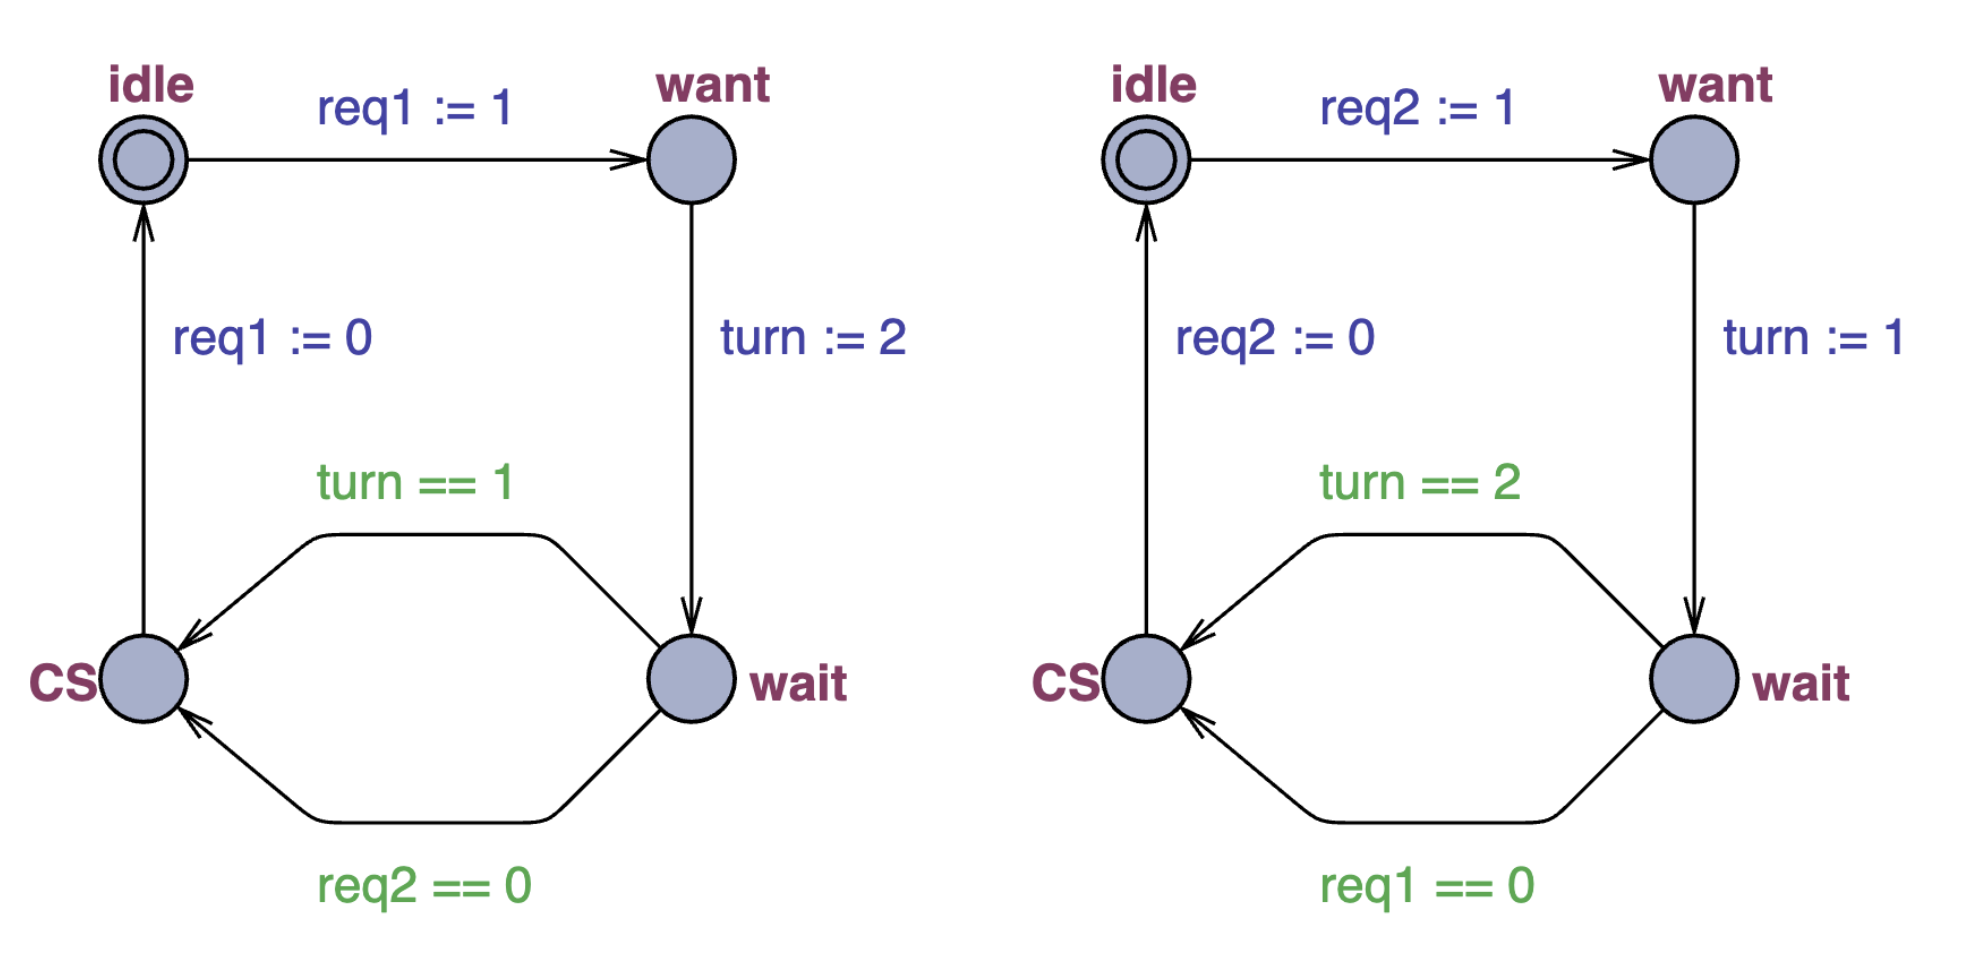
\includegraphics[width=\textwidth]{images/mutex.png}
\label{fig:mutex_uppaal}
\end{figure}

\noindent
To model Peterson's solution of the mutual exclusion algorithm we will represent two processes as separate automata. The automaton on the left in Figure \ref{fig:mutex_uppaal} will represent \texttt{Process 1} from Figure \ref{fig:mutex_code} and the right automaton will represent \texttt{Process 2}. Both automata have the same set of locations, namely, \texttt{idle}, \texttt{want}, \texttt{wait}, and \texttt{CS}. Location \texttt{idle} represents the state of the process in which it does not request access to the critical section. Location \texttt{want} represents the state of the process after requesting access to the critical section. Location \texttt{wait} indicates that the process set the turn to access the critical section to the other process. Automaton will remain in location \texttt{wait} until one of the guard conditions gets satisfied and enables the transition to location \texttt{CS}. Location \texttt{CS} is a critical section of the process. Upon transition from location \texttt{CS} to \texttt{idle} a process will no longer request access to the critical section. 


\subsection{Verifying properties in UPPAAL}

% Logical quantifiers in UPPAAL
\begin{definition}[Logical quantifiers in UPPAAL \cite{Bengtsson2004}]
The formulas should be one of the following forms\\
- \texttt{A[]$\phi$} -- Invariantly $\phi$.\\
- \texttt{E<> $\phi$} -- Possibly $\phi$.\\
- \texttt{A<> $\phi$} -- Always Eventually $\phi$.\\
- \texttt{E[] $\phi$} -- Potentially Always $\phi$.\\
- \texttt{$\phi$ --> $\psi$} -- $\phi$ always leads to $\psi$.\\
where $\phi, \psi$ are local properties that can be checked locally on a state, i.e. boolean expressions over predicates on locations and integer variables, and clock constraints.
\label{def:quantifiers}
\end{definition}


% Successfully verified properties for mutex
\begin{figure}[H]
\caption{Successfully verified properties for mutex \cite{SmallTutorial2009}}
\label{fig:mutex_verification}
\begin{lstlisting}[style=code]
A[] not (P1.CS and P2.CS)
E<> P1.CS
E<> P2.CS
\end{lstlisting}    
\end{figure}
\section{Methods}
In the literature there are multiple approaches for verification and testing of implemented swarm behaviours. There are several works which document algorithms for those behaviours with the related experiments and results \cite{Formal_Verification_of_Probabilistic_Swarm_Behaviours},\cite{Towards_Temporal_Verification_of_Emergent_Behaviours_in_Swarm_Robotic_Systems}, \cite{Property-driven_design_for_swarm_robotics}. In some cases there is an automaton corresponding to the textual description of behaviour or pseudocode \cite{Formal_Verification_of_Probabilistic_Swarm_Behaviours}. At times, used logic and tools are mentioned \cite{Property-driven_design_for_swarm_robotics}. However we are not be able to reproduce the experiments because none of the works explained in detail how the chosen swarm behaviour was modelled. That is why this section will focus on explaining how algorithm's pseudocode and general assumptions are transformed into a functioning model. The selected algorithm to demonstrate the process of modelling is Alpha algorithm. It was chosen because there were many experiments that addressed Alpha algorithm but omitted the details of what was actually being tested or verified \cite{Towards_Temporal_Verification_of_Emergent_Behaviours_in_Swarm_Robotic_Systems}, \cite{On_Formal_Specification_of_Emergent_Behaviours_in_Swarm_Robotic_Systems}.

\subsection{Alpha algorithm}
Alpha algorithm was introduced by Julien Nembrini in \cite{Minimalist_Coherent_Swarming_of_Wireless_Networked_Autonomous_Mobile_Robots}. It was inspired by Kasper Støy's work \cite{Using_Situated_Communication_in_Distributed_Autonomous_Mobile_Robotics}. Støy proposed and implemented a simple control system for aggregating robots. Instead of relying on environment and localisation information, it uses physical properties of the signal used for communication. Robot behaviour is solely determined by the change in the number of robots that are in the range of its signal.

Alpha algorithm is an approach to an aggregation task within the category of spatial organisation. It is based on the assumption that robots send and receive signals through omnidirectional channels like radio or infrared. Single robots make decisions about their movement only based on the number of connections to other robots. The inter-connectivity of the swarm is controlled by the alpha parameter which is a threshold on the desired number of connections for a single robot. Pseudocode defining the Alpha algorithm can be found in Figure \ref{fig:pseudocode}. Variable \textbf{i} in the pseudocode is a loop iterator and \textbf{cadence} is a parameter that controls how often a robot will send its ID and check the number of neighbours.

In order to explain the Alpha algorithm in a greater detail we will divide the most important aspects of the robot behaviour into subsections. First three subsections, namely, Movement, Connection, Initialisation and clocks, will explain the algorithm's general assumptions and design choices. The fourth and last subsection - Automaton, will transform the pseudocode for the Alpha algorithm into timed automaton while incorporating design choices introduced in previous subsections.

\begin{figure}[H]
\caption{Pseudocode for Alpha algorithm from \cite{Minimalist_Coherent_Swarming_of_Wireless_Networked_Autonomous_Mobile_Robots}}
\begin{lstlisting}
Create a list of neighbours for robot, Nlist
k = number of neighours in Nlist
i = 0

loop forever {
	i = i modulo cadence

	if (i = 0){
		Send ID message

		Save copy of k in LastK
		k = number of neighbours in Nlist

		if ((k < lastK) and (k < alpha)){
			turn robot through 180 degrees
		}
		else if (k > LastK) {
			make random turn
		}
	}

	Steer the robot according to state
	Listen for calls from robots in range
	Grow Nlist with neighbours IDs

	i++
}
\end{lstlisting}
\label{fig:pseudocode}
\end{figure}


\subsection{Movement}
There would be no need for Alpha algorithm without the robot movement so it is important to define how it is modelled. Robot always moves in one of four directions: up, right, down or left. Initial direction is chosen at random and mapped to vertical and horizontal components. Direction will not change unless the robot performs random turn or 180 degree turn. Random turn chooses new direction in the same way that initial direction is determined. This means that random turn may result in maintaining the current direction of the robot with approximately 25\% chance. 

Robot movement is achieved by incrementing the robot's coordinates with vertical and horizontal direction components. Direction component values are  $\in \{-1, 0, 1\}$, but either vertical or horizontal direction component has to be equal to zero. This means that robot will move in one of four possible directions with a step size equal to one. Every time the robot moves, it will update its coordinates in the globally available data structure. Environment in which robot exists is an unbounded grid that can be continuously traversed in four directions.

Robots are not aware of other robots positions. This means that they can occupy exactly the same point of the grid. Additionally, there is no collision avoidance mechanism that would prevent them from crashing into each other while moving. This simplification could be eliminated but at the cost of implementation being further apart from the original idea of what is an Alpha algorithm. We would have to make arbitrary decisions about robot behaviour in the case of collision or inability to move to the occupied point on the grid.

\subsection{Connection}
Number of robot connections is the main parameter determining the robot behaviour. Therefore it is important to accurately model what it means for robots to be connected. One of the assumptions in Julien Nembrini's \cite{Minimalist_Coherent_Swarming_of_Wireless_Networked_Autonomous_Mobile_Robots} is that physical signal is omnidirectional. However, robot movement is modelled to be two dimensional. Consequently we will assume that two robots are connected if their distance is smaller than radius of physical signal that we mimic. Length of the radius will determine how far apart the robots can move before losing connection.

To model the physical signal we need information about robot coordinates, mutual distances, previous and current number of neighbours. This allows for evaluating whether robots are in the signal distance and therefore connected or not. Every time robot moves it will update its own coordinates, previous number of neighbours for itself, current number of neighbours for all robots and mutual distances for all robots. It may seem like the robot is using more information than it is assumed in the Alpha algorithm. Information that it passes is used to mimic the physical signal of the real robot. Although, it updates its coordinates, robot is not aware of the position of its neighbours. Its movement is derived solely from information about previous and current number of neighbours. 

The desired number of connections is set by the alpha parameter. If the number of connections falls below alpha, robot will react and turn 180 degrees in order to try to reconnect with other robots. Alpha parameter influences connectivity of the swarm. If the parameter is set to higher values the robots will try to maintain more connections and the resulting swarm will be more compact. If the parameter is set to lower values, robots will be able to move further apart as they will need to maintain less connections. What is low and high value for alpha parameter is subjective to the size of the swarm.

\subsection{Initialisation and clocks}
This subsection explains the initial state of the robot and the influence that the time has on its behaviour. Every robot gets initialised with the same set of parameters apart from its ID. In the beginning all robots are placed at exactly the same point. They have no direction until transitioning to the next state - RANDOM STATE, and will not move forward until transitioning further. In the INITIAL state robots cannot access information about number of current neighbours and number of last neighbours. The INITIAL state becomes unreachable after the robot transitions from it.

Pseudocode variables \textbf{i} and \textbf{cadence} model the frequency of robot actions. Specifically \textbf{cadence}, it controls how often a robot sends a signal and checks if it should change direction. While we are able to model such frequency without a timed automaton we would not be able to model a real-time system like robot swarm. The timing aspect allows us to model a system with time dependent behaviours and to verify a time dependent properties. We can observe a system behaviour throughout time and evaluate the stability of the implemented algorithm. That is why each robot has its own clock that controls how long it can remain in the current state before being forced to transition. After each transition to the next state the robot will reset its own clock. Maximum time for the robot to remain in state can influence the behaviour of the whole system. If we decrease the maximum time of inactivity, we will obtain a system that is on average more reactive and even. With increasing the maximum time of inactivity we increase the chances of robots operating in different pace. As we are modelling swarm we should aim for uniform operation and therefore lower maximum times for inactivity.

\subsection{Automaton}
In order to implement the Alpha algorithm presented in \cite{Minimalist_Coherent_Swarming_of_Wireless_Networked_Autonomous_Mobile_Robots}, we utilised the pseudocode from Figure \ref{fig:pseudocode}, with design choices described in the previous subsections. The implementation is a timed automaton - Figure \ref{fig:automaton}.

We will describe how pseudocode was mapped into the timed automaton. Pseudocode starts with creating and initialising variables that are needed for algorithm execution. This part is not explicitly visible in the automaton but achieved during initialisation of the model.\\\\
Pseudocode variables that represent the state:\\
- \textbf{Nlist}, a list of neighbours for a robot;\\
- \textbf{ID}, a unique robot identifier;\\
- \textbf{k}, a number of neighbours in Nlist;\\
- \textbf{lastK}, a previous number of neighbours in Nlist;\\
- \textbf{alpha}, a threshold on the number of connections;\\

 The state of the algorithm before entering the infinite loop is represented by the INITIAL state. Transitioning from the INITIAL state is equivalent to entering the infinite loop defined in the pseudocode. The entry point for the loop is a RANDOM TURN state where the robot obtains its initial random direction. Infinite loop defines that robot will send its ID and make a decision about turning only every 'cadence' loop iterations. To mimic this behaviour cadence was implemented as the maximum time of inactivity $T$. In the pseudocode  decision about turning is realised with 'if' and 'if else' statements. Statements and their corresponding conditions were transformed to IF and IF ELSE states with conditions guarding subsequent transitions. Guarded transitions utilise original conditions and their negations. In this way we can guarantee that there is always only one transition possible at any point. Variables used in the conditions correspond to the current number of neighbours, previous number of neighbours and desired number of neighbours. Those variables control the behaviour of a single robot alongside the maximum time of inactivity $T$ which acts as a cadence parameter of the loop. Single robot is represented by the timed automaton presented in Figure \ref{fig:automaton}. Composition of such timed automata results in a robot swarm implementation of the Alpha algorithm. The movement and interactions of robots cause them to update their variables. Those variables are then used to determine the logical value of conditions guarding the state transitions. Finally, the available transitions are taken, influencing the robots behaviours. This process restarts and lasts indefinitely as the system composed of timed automata has no final state.\\

\noindent State descriptions:\\
- INITIAL, where the robot is not moving and has no direction;\\
- RANDOM TURN, where the robot randomly chooses one of four directions;\\
- U-TURN, where the robot changes direction by 180 degrees;\\
- FORWARD, where the robot moves forward in the set direction;\\
- IF, where the robot checks if it is disconnected from neighbours;\\
- ELSE IF, where the robot checks if it is connected to more than desired number of neighbours;\\\\
States are not enough to define the behaviour if the robot is not forced to transition. Each robot has its own clock that controls how much time it can remain in a given state. Time - $t$ a robot can remain in states FORWARD and INITIAL is limited by the maximum time $T$.
Robot has to transition before time $t$ is equal to $T$. After leaving mentioned states, the robot resets its clock. In remaining states the time doesn't pass and therefore time $t$ is not incremented. However other transitions are guarder by associated conditions. Transition from one state into another can only happen if the corresponding condition is satisfied. If there is no condition over the edge, transition can always be taken.\\\\ Conditions controlling the robot are associated with the following variables:\\
$n$ - current number of neighbours;\\
$l$ - previous number of neighbours;\\
$\alpha$ - Alpha parameter, desired number of neighbours;\\
\begin{figure}[H]
\caption{Timed automaton for the Alpha algorithm}
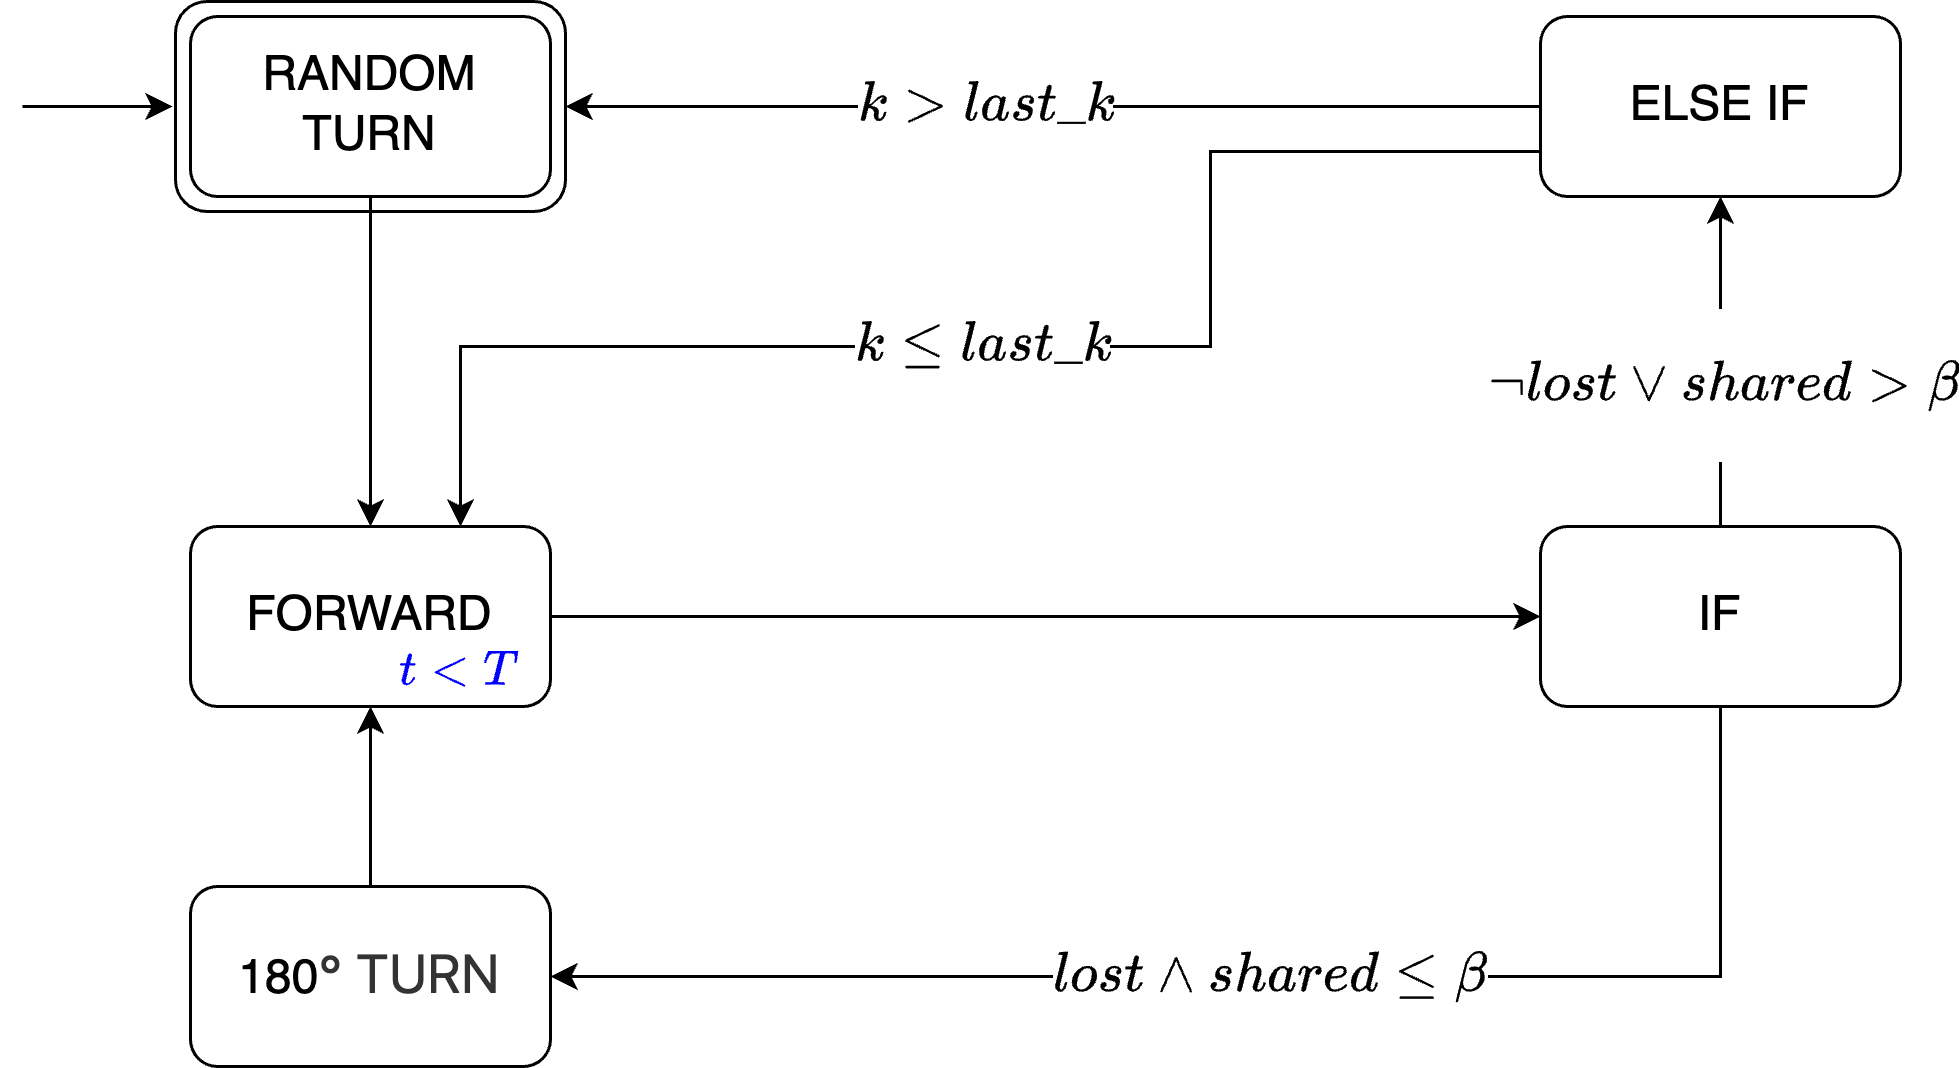
\includegraphics[scale=0.9]{images/automaton.png}
\label{fig:automaton}
\end{figure}
\section{Implementation}
In this section, we will describe the implementation of the timed automaton model from the previous section, shown in Figure \ref{fig:automaton}. Our tool of choice is UPPAAL, an integrated solution for modeling, simulation, and verification of timed automata. We will present the implementation of limitations imposed on the model in the following subsection.  Model variables representing its state will be described along with the most important functions.


\subsection{Model}
Implementation of the timed automaton, shown in Figure \ref{fig:implementation}, has an additional state called \texttt{grid} and global functions that abstract away the underneath complexity. This state is a consequence of imposing limitations on the environment size defined in the previous section. This allows us to reduce the state space size and perform verification. It is the biggest change made to the original algorithm, defined in Figure \ref{fig:pseudocode}. In that state, it is determined whether a robot has reached the boundary of the grid. If yes, the robot will transition to the state \texttt{turn\_180} and change its direction by 180 degrees as it cannot continue moving forward outside of its environment. If a robot has not reached the boundary of its environment it will transition to the \texttt{if} state where it will follow the original rules of the algorithm.

\begin{figure}[H]
\caption{Asynchronous implementation of the Beta algorithm}
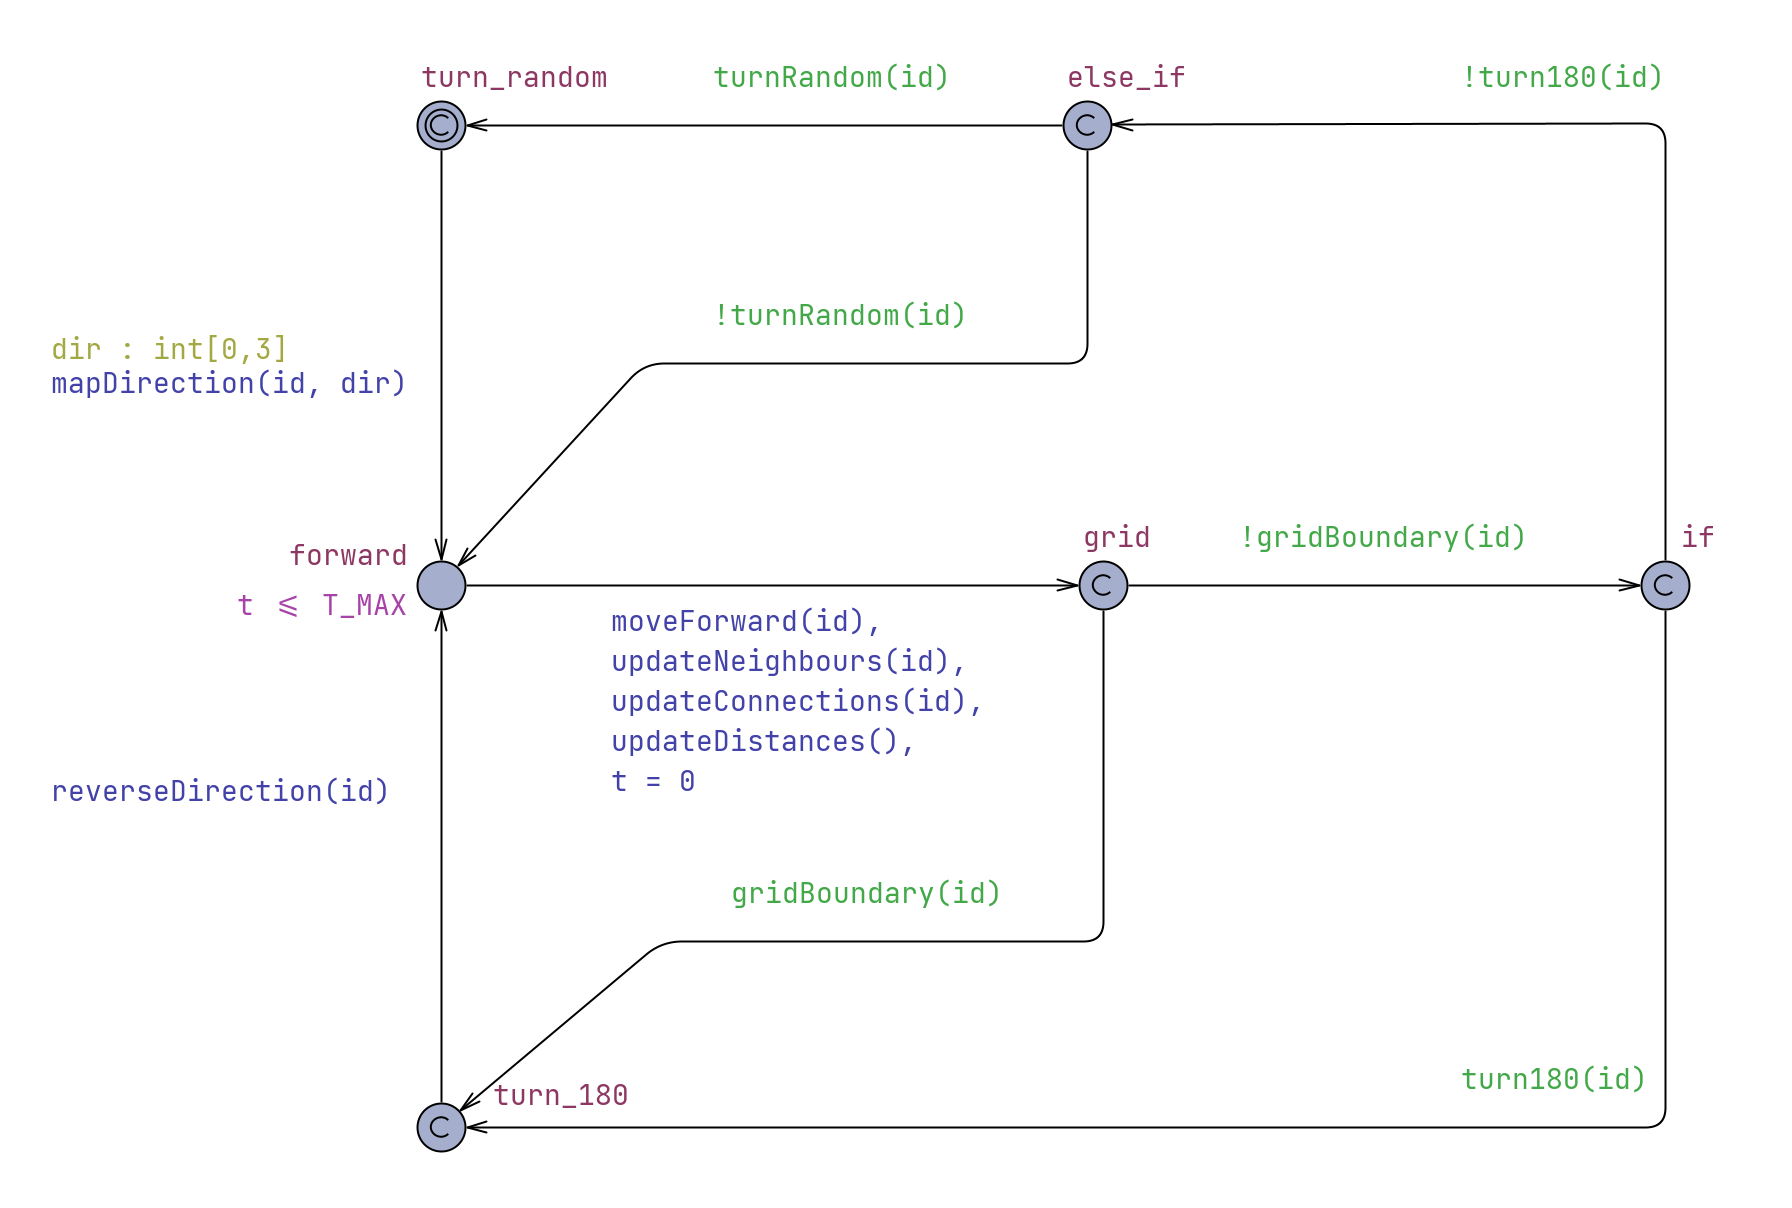
\includegraphics[width=\textwidth]{images/implementation.png}
\label{fig:implementation}
\end{figure}

\noindent
Implementation presented in Figure \ref{fig:implementation} is asynchronous. Robots can move at different pace and time, independent of each other. We also implemented a synchronised version of the Beta algorithm to investigate the influence of the mode of concurrency on verification results. The synchronised implementation is presented in Figure \ref{fig:implementation_synchronised}, and its synchronisation mechanism in Figure \ref{fig:implementation_synchronised_barrier},

\begin{figure}[H]
\caption{Synchronised implementation of the Beta algorithm}
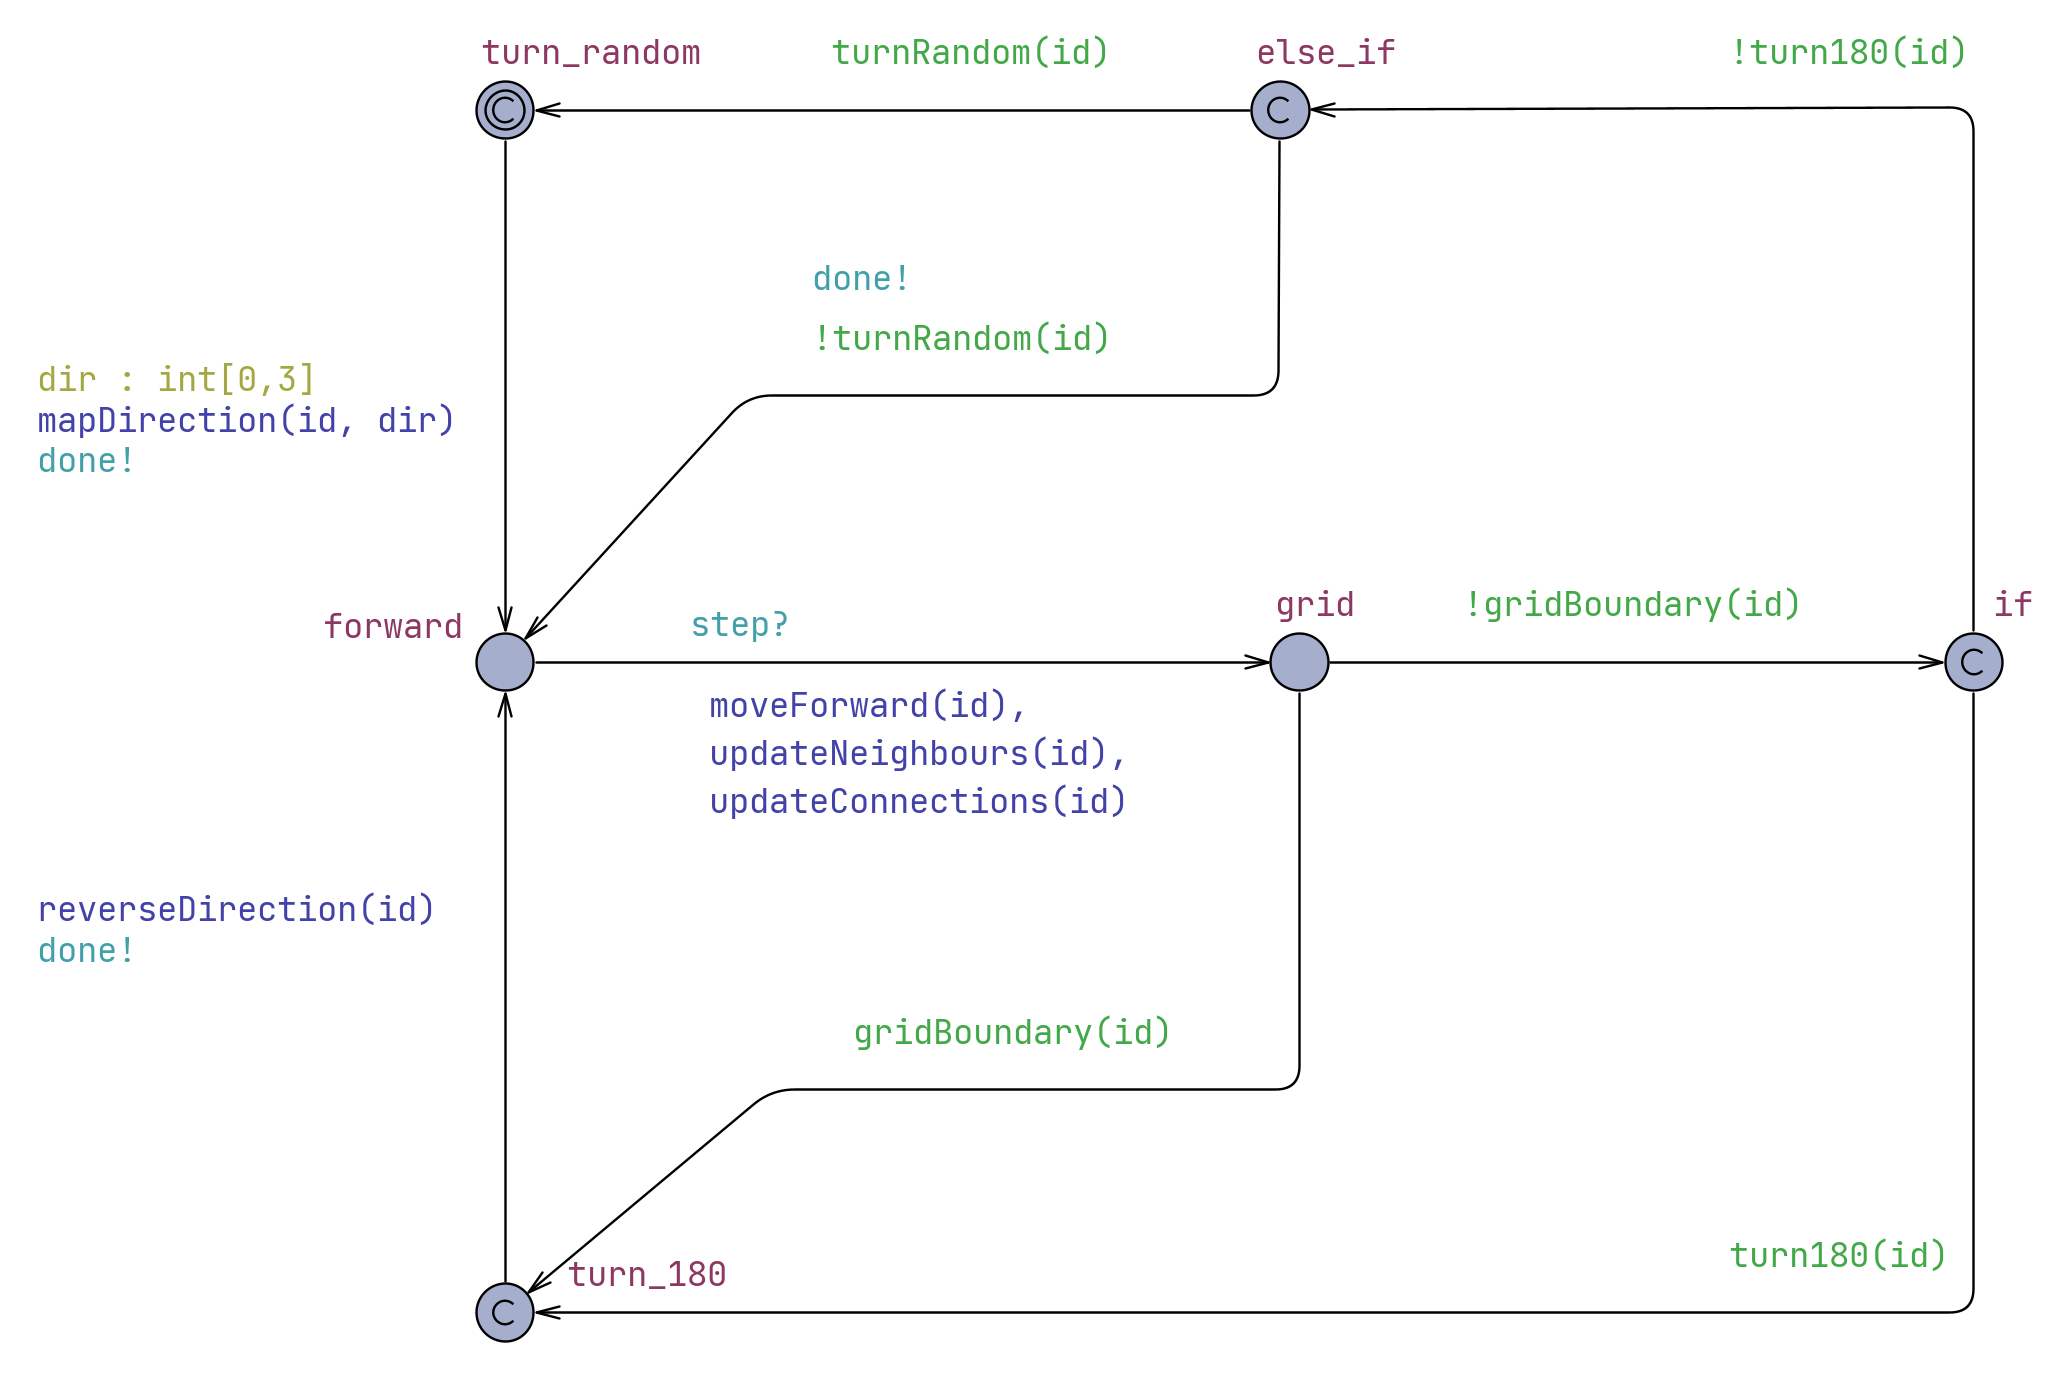
\includegraphics[width=\textwidth]{images/implementation_synchronised.png}
\label{fig:implementation_synchronised}
\end{figure}

\begin{figure}[H]
\caption{Synchronisation mechanism}
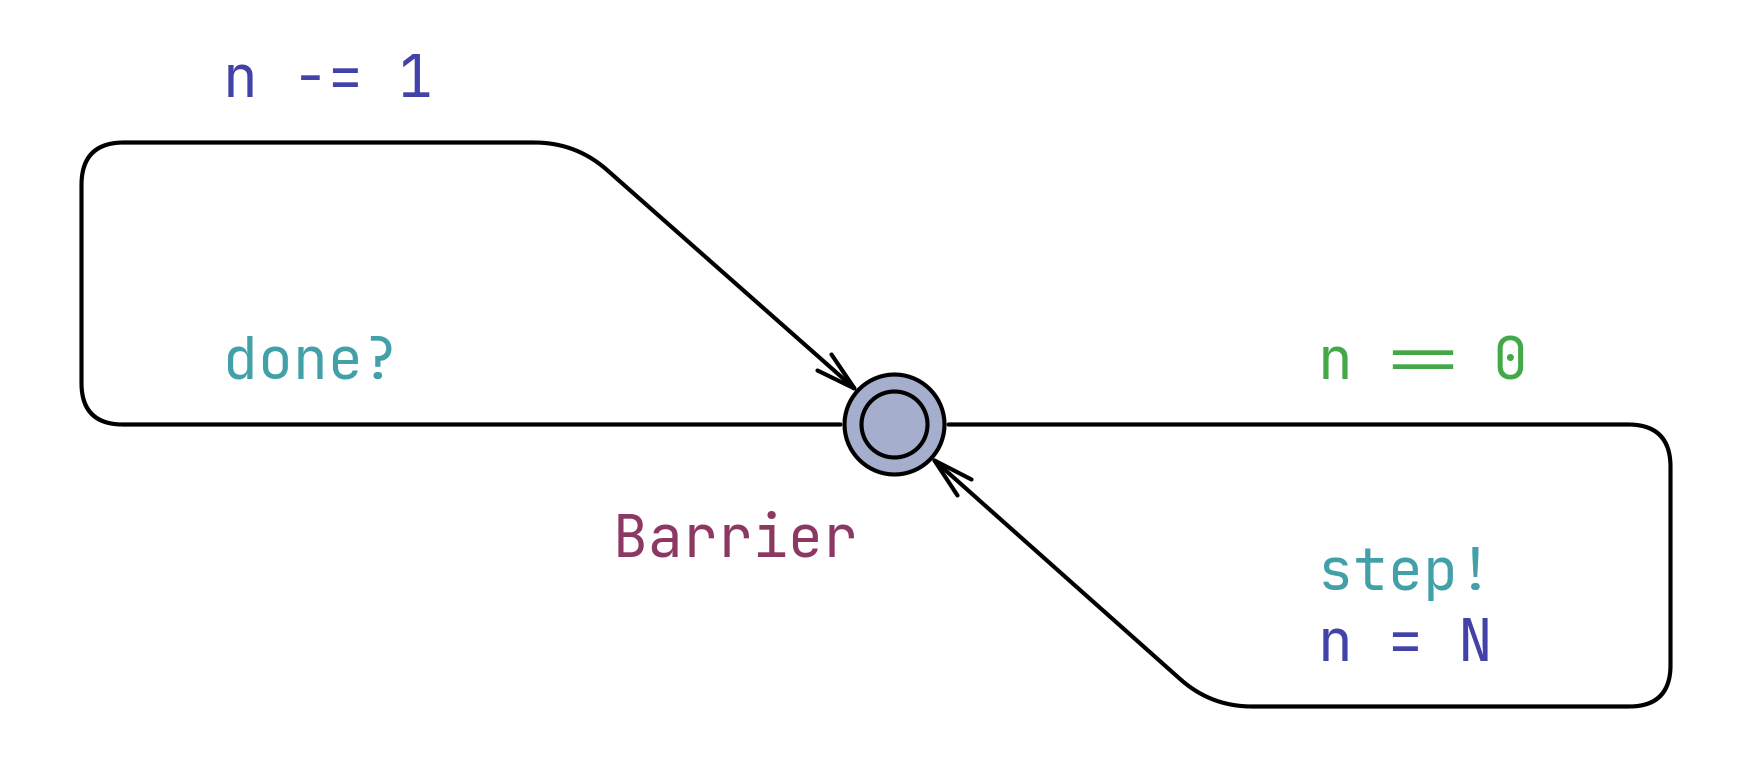
\includegraphics[width=\textwidth]{images/implementation_synchronised_barrier.png}
\label{fig:implementation_synchronised_barrier}
\end{figure}

\subsection{Movement}



\subsection{Connection}



\subsection{System variables}

\section{Results}
\subsection{Verifying implementation}
In this section we will present verification results for implementation and the Beta algorithm for two modes of concurrency. The first mode of concurrency is asynchrony which is the intended mode for the Beta algorithm. The second implementation is synchronised to verify the influence of the concurrency mode on algorithm effectiveness. In the asynchronous case, presented in Figure \ref{fig:implementation}, robots can move at different rates. Each robot is forced to move from \texttt{forward} location after \texttt{T\_MAX} amount of time but can also transition sooner. In the synchronised implementation, presented in Figures \ref{fig:implementation_synchronised} and \ref{fig:implementation_synchronised_barrier}, all robots are forced to move at the same time. By verifying algorithm specific properties we will show the influence of the mode of concurrency on algorithm effectiveness in maintaining swarm coherence.

% System specification
\begin{figure}[H]
\caption{System specification for asynchronous implementation}
\label{fig:implementation_asynchronous_system}
\begin{lstlisting}[style=code]
N = 2;      // Number of robots
R = 1;      // Signal radius
STEP = 1;   // Step size
BETA = 1;   // Beta parameter
G = 3;      // Grid boundary
T_MAX = 1;  // Time threshold
\end{lstlisting}
\end{figure}

% Properties
\begin{figure}[H]
\caption{Successfully verified properties for synchronous implementation}
\label{fig:implementation_asynchronous_properties}
\begin{lstlisting}[style=code]
1. A[] forall(i : int[0, N-1]) x[i] != G or y[i] != G
2. A[] forall(i : int[0, N-1]) abs(x[i]) <= G && abs(y[i]) <= G
3. E<> C > 0 && P0.turn_random
4. E<> C > 0 && P0.turn_180
5. A[] P0.forward imply P0.t <= T_MAX
6. E<> P0.turn_180 && abs(x[0]) != G && abs(y[0]) != G 
7. E<> P0.turn_180 && (abs(x[0]) == G || abs(y[0]) == G)
8. E<> P0.forward && k[0] <= last_k[0]
9. A[] P0.t != 0 imply P0.forward
10. A[] (P0.turn_random or P0.turn_180 or P0.grid or P0.grid or P0.if or P0.else_if) imply P0.t == 0
11. A[] forall(i : int[0, N-1]) shared_neighbours[i][0] == 0 and shared_neighbours[i][1] == 0
12. A[] forall(i : int[0, N-1]) C < 0 imply k[i] == N-1
13. A[] forall(i : int[0, N-1]) C > 0 imply x_dir[i] != 0 or y_dir[i] != 0
14. A[] not deadlock
\end{lstlisting}    
\end{figure}

\noindent
Explanation of properties from Figure \ref{fig:implementation_asynchronous_properties}:\\
1. For all the paths through the system, no robot can have their x and y coordinate equal to the grid boundary at the same time. No robot will ever reach the corner of the grid.\\
2. For all the paths through the system, all robots will stay within grid boundaries.\\
3. There exists a path through the system, for a robot to reach location \texttt{turn\_random} after initialization. This means that following locations are reachable: \texttt{forward}, \texttt{grid}, \texttt{if}, \texttt{else\_if}. It also means that following transitions are reachable: \texttt{turn\_random} $\rightarrow$ \texttt{forward}, \texttt{forward}n $\rightarrow$ \texttt{grid}, \texttt{grid} $\rightarrow$ \texttt{if}, \texttt{if} $\rightarrow$ \texttt{else\_if}, \texttt{else\_if} $\rightarrow$ \texttt{turn\_random}.\\ 
4. There exists a path through the system, for a robot to reach location \texttt{turn\_180} after initialization.\\
5. For all the paths through the system, a robot will obey the invariant on location \texttt{forward}.\\
6. There exist a path through the system, for a robot to reach location \texttt{turn\_180} without reaching the boundary of the grid. This means that transition from \texttt{if} to \texttt{turn\_180} is reachable.\\
7. There exist a path through the system, for a robot to reach location \texttt{turn\_180} as a result of reaching the boundary of the grid. This means that transition from \texttt{grid} to \texttt{turn\_180} is reachable.\\
8. THIS PROPERTY MIGHT NOT BE STRONG ENOUGH.\\
9. For all the paths through the system, robot's clock value different than zero implies it being in the \texttt{forward} location. This means that time perceived by the robot is only allowed to pass in the \texttt{forward} location.\\
10. For all the paths through the system, a robot presence in the listed location imply that its clock value is equal to zero. For the robot, time will not pass in any other location than forward.\\
11. For all the paths thorugh the system, two robots will not share a neighbor. This is a consequence of a fact that in the system consisting of two robots, they cannot have a neighbor in common.\\
12. For all paths through the system, all robots are fully connected as part of system initialization.\\
13. For all paths through the system, all robots have their directions set after system initialization.\\
14. There is no path through the system, which will results in deadlock.\\





\subsection{Verifying the algorithm}

\section{Discussion}
Verification of the Beta algorithm for the asynchronous implementation showed that the algorithm coherence is not guaranteed for the Beta parameter equal to two. That value was used in the original paper \cite{Nembrini2002} however, other values of the Beta parameter were used but their influence was not examined. For swarms of size three, it was shown that all of the robots can become disconnected for at least two steps. For swarms of size four, it was shown that a single robot can become disconnected for at least two steps. The diagnostic trace produced upon verification of property defined in figure \ref{fig:algorithm_asynchronous_properties_2}, was used as a starting point for manual traversal through possible system states using UPPAAL's symbolic simulator. This led to the exploration of positive and negative scenarios for the swarm presented in Figures \ref{fig:lost_connection} and \ref{fig:reconnection}. Due to hardware limitations, it was not possible to verify whether a swarm consisting of four robots could become fully disconnected for at least two steps.
\\\\
While the swarm will react to the formation of bridges described in the original paper \cite{Nembrini2002}, it will not prevent them from forming. This can be observed in the scenario presented in Figure \ref{fig:lost_connection}. This can be partially attributed to the concurrency mode used by the system. Property that describes the situation of a single robot becoming disconnected from the swarm for at least two steps was verified as true for the system operating in asynchronous mode and falsified for the synchronized system. By examining scenarios presented in Figures \ref{fig:lost_connection} and \ref{fig:reconnection} one can speculate that robots that operate in similar frequency are more likely to reconnect. If robots operated in a more uniform way it could be easier for them to reconnect. In the situation of asynchrony, a group of robots may move away before the lost robot realizes that it is disconnected. 
\\\\
When verifying properties of the Beta algorithm for the synchronized system it was found that all of the robots can become disconnected for a single step. However, it was also found that a single robot can't become disconnected for two or more steps. Properties that were verified and falsified can be found in Figures \ref{fig:algorithm_synchronised_properties_true} and \ref{fig:algorithm_synchronised_properties_false}. It can be argued that one of the reasons for this outcome is the reactivity of the system in which all robots move forward at the same time. This could be treated as an indication that the uniformity of robot operations might be a crucial aspect of the algorithm. 
\\\\
There were several limitations affecting the verification process and results, the most significant being the state-space explosion problem. A swarm of size four produced too many states for full verification on a single laptop. To make verification possible, the grid was bounded, and the robot algorithm modified: robots performed a 180-degree turn upon reaching the grid's boundary. This altered the original algorithm and affected its effectiveness, as robots could reconnect by bouncing off boundaries. As a result, defining a property to detect a disconnected robot was straightforward unlike defining one for a connected swarm that did not become connected as a result of interacting with the boundary.
\section{Conclusions}
In this paper, we have presented the process of modeling, implementing, and verifying the Beta algorithm for a robot swarm using timed automata and UPPAAL. Through the implementation and verification of both asynchronous and synchronized implementations, we highlighted the influence of the concurrency mode on the algorithm's effectiveness in maintaining swarm coherence. While the Beta algorithm demonstrated responsiveness to lost connections, challenges emerged in guaranteeing reconnection in the asynchronous system. Furthermore, the reconnection of the swarm cannot be attributed solely to the Beta algorithm, as it is also influenced by the limited area of the grid. These insights highlight the difficulties in verifying swarm robotic algorithms and the influence of robot uniformity on the effectiveness of the algorithm.
\\\\
The results of our verification showed that the synchronization mode significantly affects the coherence of the swarm. Synchronized implementations completely eliminated prolonged disconnections. While this demonstrated the importance of uniformity in robot behavior for maintaining connectivity, a fully synchronized solution defeats the most basic assumption of swarm robotics: decentralization. In contrast, asynchronous systems, while aligning more closely with real-world scenarios, faced challenges with timely reconnection. Additionally, the bounded grid environment introduced limitations that, while necessary for computational feasibility, influenced the outcomes of the algorithm. This highlights the need to balance practical constraints with algorithmic integrity when implementing and verifying swarm robotics algorithms.
\\\\
Future work should focus on developing additional properties to verify the Beta algorithm, ensuring a more comprehensive understanding of its behavior under various conditions. Exploring other approaches to limiting the grid, such as implementing different boundary behaviors or using varying grid sizes, could provide more flexibility in verification while maintaining computational feasibility. Additionally, verification should be expanded to larger swarms with different parameter values, such as varying the Beta parameter and robot count, to assess the algorithm’s scalability. Furthermore, a new mode could be explored where robots are not fully synchronized but operate at the same frequency, balancing the benefits of both presented implementations. This would provide valuable insights into the algorithm's effectiveness.





% bibliography
\bibliography{refs}
\bibliographystyle{plain}


\end{document}
